\begingroup
\linespread{1}\selectfont
\resizebox{\linewidth}{!}{%
\begin{tikzpicture}[x=1pt,y=-1pt]
\node[anchor=north west,inner sep=0pt,outer sep=0pt] at (0,0) {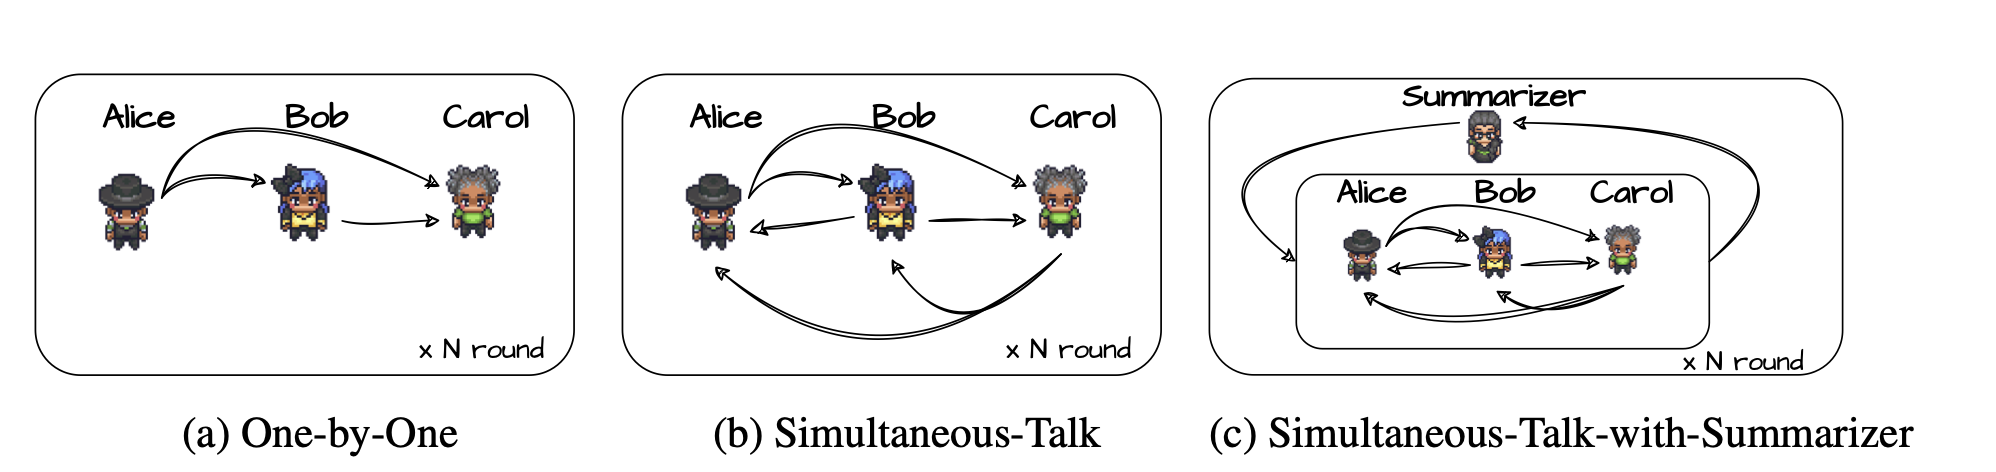
\includegraphics[width=1996pt]{figures/chateval.png}};
\fill[fill=white] (1392,81) rectangle (1616,111);
\fill[fill=white] (1270,87) rectangle (1445,126);
\node[anchor=center,inner sep=0pt,outer sep=0pt,align=center,text width=169pt,text=black,font={\fontsize{33.4152}{38.0933}\selectfont\sffamily\bfseries}] at (1357.5,106.5) {总结器};
\fill[fill=white] (1678,349) rectangle (1831,372);
\fill[fill=white] (380,334) rectangle (554,367);
\node[anchor=center,inner sep=0pt,outer sep=0pt,align=center,text width=168pt,text=black,font={\fontsize{36.0884}{41.1408}\selectfont\sffamily}] at (467,350.5) {重复 $N$ 轮};
\fill[fill=white] (965,334) rectangle (1139,367);
\node[anchor=center,inner sep=0pt,outer sep=0pt,align=center,text width=168pt,text=black,font={\fontsize{36.0884}{41.1408}\selectfont\sffamily}] at (1052,350.5) {重复 $N$ 轮};
\fill[fill=white] (1718,267) rectangle (1827,333);
\node[anchor=center,inner sep=0pt,outer sep=0pt,align=center,text width=103pt,text=black,font={\fontsize{31.1875}{35.5537}\selectfont\sffamily}] at (1772.5,300) {重复\\$N$ 轮};
\draw[draw=black,line width=1.7pt] (1797,375) .. controls (1822,375) and (1843,355) .. (1843,330);
\fill[fill=white] (143,404) rectangle (568,470);
\node[anchor=center,inner sep=0pt,outer sep=0pt,align=center,text width=419pt,text=black,font={\fontsize{46.7812}{53.3306}\selectfont\sffamily}] at (355.5,437) {(a) 逐一发言};
\fill[fill=white] (690,404) rectangle (1175,470);
\node[anchor=center,inner sep=0pt,outer sep=0pt,align=center,text width=479pt,text=black,font={\fontsize{46.7812}{53.3306}\selectfont\sffamily}] at (932.5,437) {(b) 同时发言};
\fill[fill=white] (1200,404) rectangle (1960,470);
\node[anchor=center,inner sep=0pt,outer sep=0pt,align=center,text width=754pt,text=black,font={\fontsize{46.7812}{53.3306}\selectfont\sffamily}] at (1580,437) {(c) 带总结器的同时发言};
\pgfresetboundingbox
\path[use as bounding box] (0,0) rectangle (1996,472);
\end{tikzpicture}}
\endgroup
